\documentclass[Master]{subfiles}
\begin{document}
\subsection{Non-Abelian Anyons}\label{sec:NonAbelian}
Consider two particles and their two-particle-wave function. The particles are initially in the states  $\phi_1 $ and $ \phi_2$ thus the two-particle-wave function is $\ket{\phi_1,\phi_2}$.  
When exchanging the two particles by some time evolution $U(t_i,t_f)=T_{1,2}$ the resulting state does not need to be simply the exchanged state $\ket{\phi_2,\phi_1}$. As exchanging the particles by $T_{1,2}$ is an action on the whole system and might have further implications.
$$T_{1,2}\ket{\phi_1,\phi_2} \neq \ket{\phi_2,\phi_1}$$
When we assume that the exchange of two particles is sufficiently slow not to impact any other particles and that, as implied, both particles still exist after the exchange, then all indistinguishable particles must behave as
$$T_{1,2}\ket{\phi_1,\phi_2} = \ket{e^{i \alpha} \phi_2,e^{i \beta}\phi_1}\text{.}$$
The most famous cases are Fermions and Bosons
\begin{figure}[H]
\centering
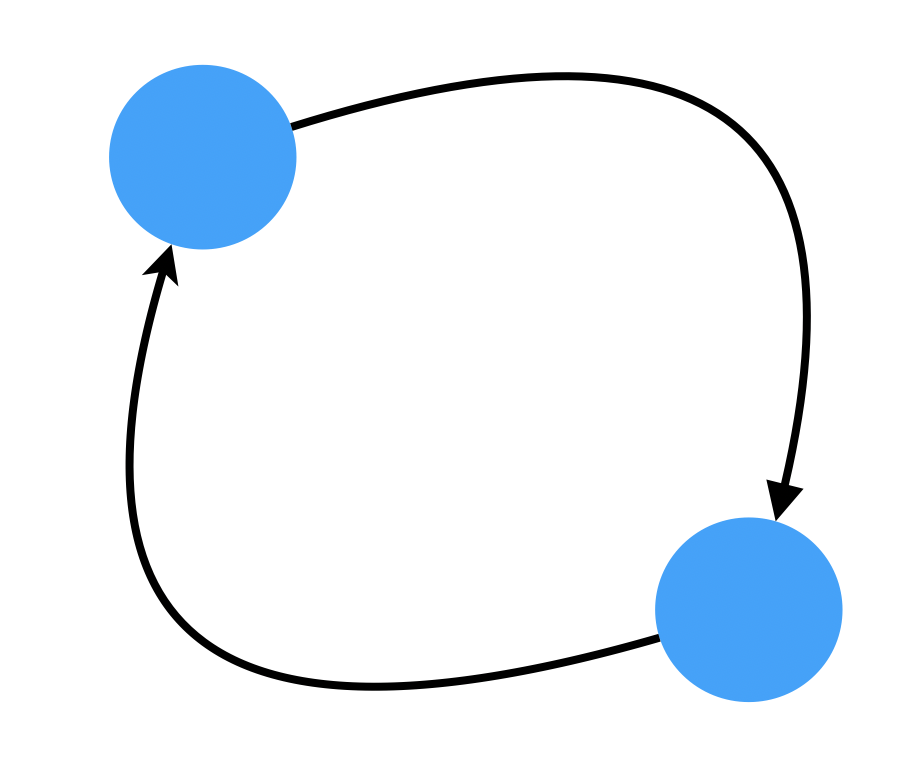
\includegraphics[width=0.3\linewidth]{imgs/Exchange.png}
  \caption{Exchange of identical particles}
  \label{fig:IdenticalExchange}
\end{figure}
Which exchange as 
$$T_{1,2}\ket{\phi_1,\phi_2} = \epsilon \ket{\phi_2,\phi_1}$$ 
with $\epsilon = +1 $ for Bosons and $\epsilon = -1 $ for Fermions. 
\subsubsection{The Different Exchange Statistics in Two and Three Dimensions}
For any dimension $\geq 3$ the spin–statistics \cite{PhysRev.58.716,} theorem shows that Fermions and Bosons are the only two possibilities.
Indeed more complicated exchange relations are possible in two dimensions. There are two intuitive ways to show why the exchange of particles in two dimensions differs from the exchange in three.
\begin{figure}[H]
\centering
\begin{minipage}{0.2\textwidth}
\centering
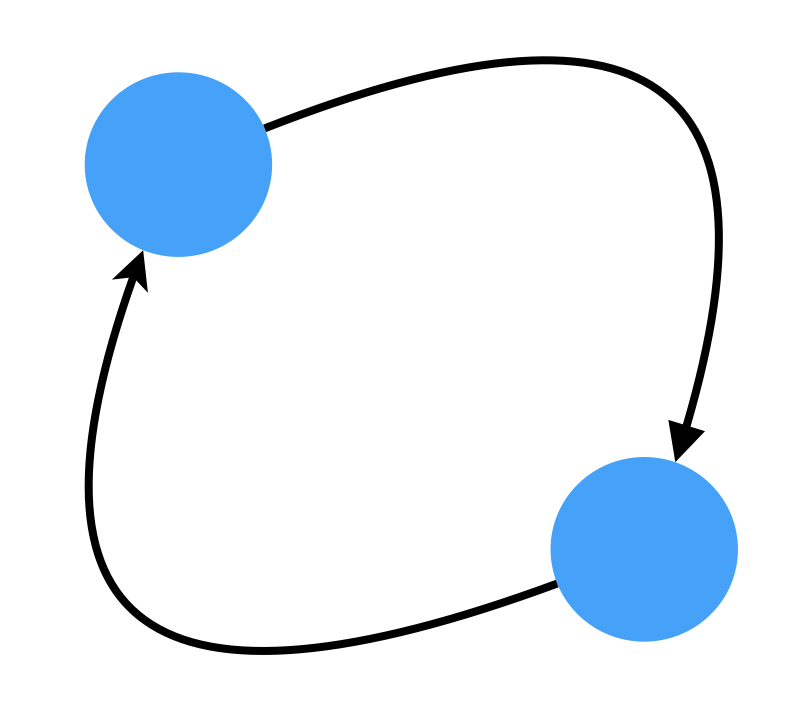
\includegraphics[width=0.5\linewidth]{imgs/AClockwhise.png}
\caption{Clockwise}
\end{minipage}
\hspace{0.5cm}
\begin{minipage}{0.2\textwidth}
\centering
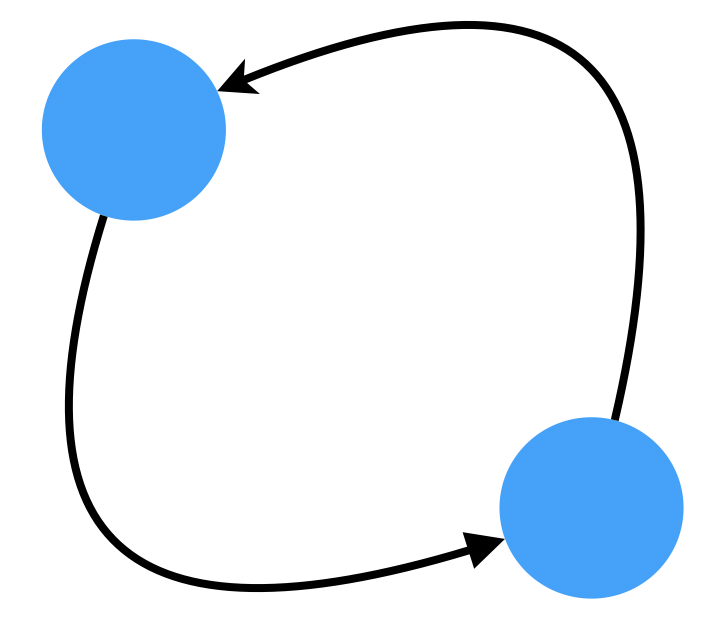
\includegraphics[width=0.5\linewidth]{imgs/Clockwhise.png}
  \caption{Counter-clockwise}
  \end{minipage}
  \hspace{0.5cm}
  \begin{minipage}{0.2\textwidth}
  \centering
  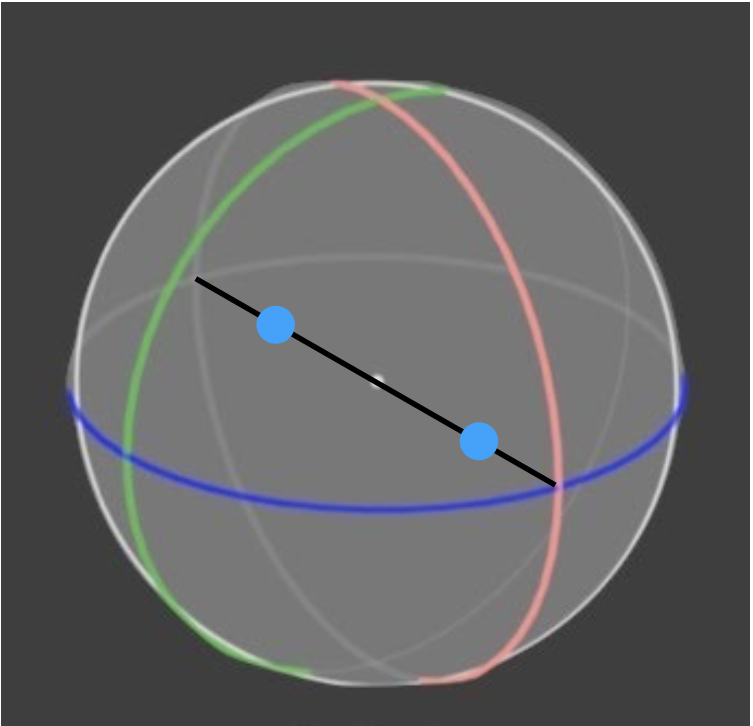
\includegraphics[width=0.5\linewidth]{imgs/RotSym2Particles.png}
\caption{Exchange of identical particles in 3D}
\end{minipage}
  \label{fig:IdenticalExchange3D}
\end{figure}
In two dimensions, there are two topologically different sets of paths exchanging two particles. One set includes a clockwise $T_{1,2}$, and one a counter-clockwise $T_{2,1}$ rotation.  The only way to deform the paths in an counter-clockwise set into a path in the clockwise set is either through a rotation in a higher dimension or two clockwise rotations, one reverting inverting initial counter-clockwise exchange.
\begin{center}
\textbf{2D} 
$$T_{1,2}\ket{\phi_1,\phi_2} \neq T_{2,1}\ket{\phi_1,\phi_2}$$
\end{center}
However, in three dimensions the clockwise and counter-clockwise connected by an out of plane rotation . This rotation is also a $SU(2)$ symmetry of the two-particle state. Therefore, the outcome of any exchange $T_{1,2}(\vec{w})$ around an Axis $\vec{w}$ must be the same for all $\vec{w}$ by the symmetry and thus for all exchange operations.
\vspace{.5cm}\\
\begin{center}
\textbf{3D}
\end{center}
\begin{equation}\label{eq:1}
\forall \vec{w},\vec{u} \in \mathbb{R}^3 : T_{1,2}(\vec{w})\ket{\phi_1,\phi_2} = T_{1,2}\vec{u}\ket{\phi_1,\phi_2}
\end{equation}

In two dimensions particles can exist for which clockwise and counter-clockwise exchange yield different outcomes. \\
The other illustrative thought experiment is to perform the exchange of the particles twice. Thus, both particles end up in their original position.
\begin{figure}[H]
\centering
\begin{minipage}{0.2\textwidth}
\centering
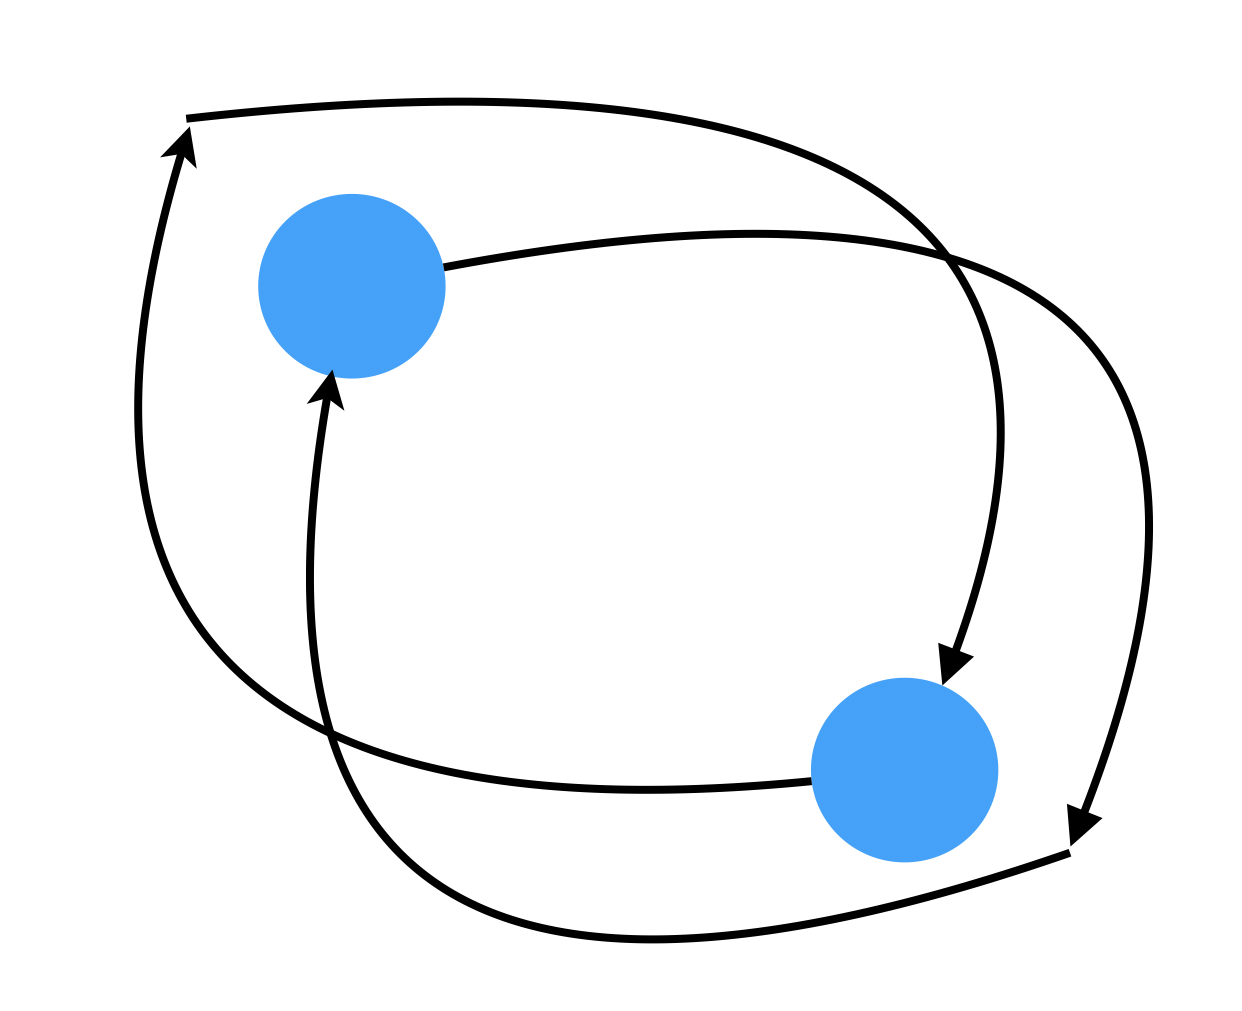
\includegraphics[width=0.5\linewidth]{imgs/DoubleExchange.png}
  \caption{Double exchange of identical particles}
  \label{fig:DoubleExchange}
  \end{minipage}
  \hspace{1cm}
  \begin{minipage}{0.2\textwidth}
\centering
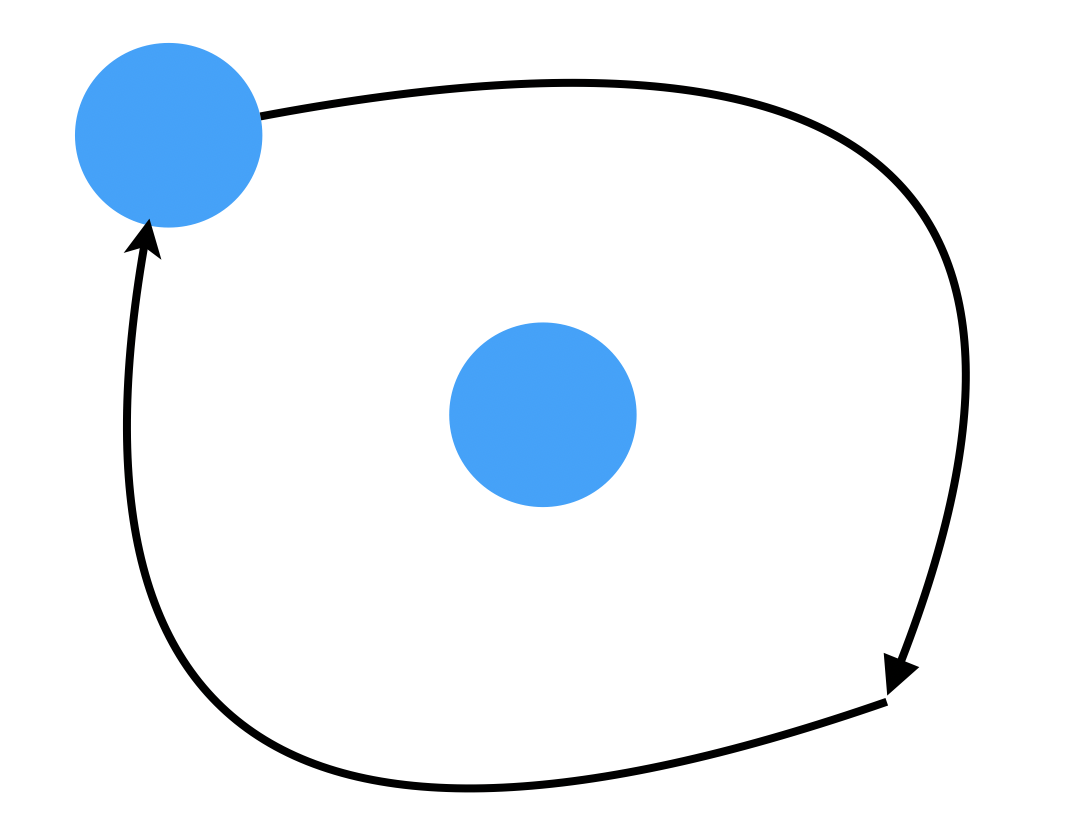
\includegraphics[width=0.5\linewidth]{imgs/TopDoubleExchange.png}
  \caption{Observed from one particle}
  \label{fig:TopDoubleExchange}
  \end{minipage}
\end{figure}
This process simplifies when viewed from the perspective of one of the two particles.  The resulting process is one particle orbiting the other. This change of perspective is equivalent to topologically deforming the paths. Only in three dimensions can we constrict the orbit above or below the orbited particle into a point. Thus, in three dimensions exchanging twice must result in the initial state.
\begin{center}
\textbf{3D} 
\begin{dmath}\label{eq:2}
T_{1,2} T_{1,2} \ket{\phi_1,\phi_2} = \ket{\phi_1,\phi_2}
\end{dmath}
\end{center}
However, in two dimensions this is not possible as we cannot constrict the path of the orbiting particle without crossing the central particle.
\begin{center}
\textbf{2D} 
$$  T_{1,2}T_{1,2}\ket{\phi_1,\phi_2} \neq \ket{\phi_1,\phi_2}$$
\end{center}
Indeed, there are examples for this behaviour in two dimensions.
However, for three dimensions we can now argue for that only Fermions and Bosons can exist.
We start with the argument for indistinguishable particles
$$T_{1,2}\ket{\phi_1,\phi_2} = \ket{e^{i \alpha} \phi_2,e^{i \beta}\phi_1}\\$$
and use \eqref{eq:1}
$$\ket{e^{i \alpha} \phi_2,e^{i \beta}\phi_1}  = T_{1,2}\ket{\phi_1,\phi_2} =  T_{2,1}\ket{\phi_1,\phi_2} = \ket{e^{i \beta} \phi_2,e^{i \alpha}\phi_1} $$ 
$$\Rightarrow \alpha = \beta$$
We can now use \eqref{eq:2}
$$T_{1,2}T_{1,2}\ket{\phi_1,\phi_2} = e^{i 2 \alpha}\ket{\phi_1,\phi_2}   = \ket{\phi_1,\phi_2} $$
$$ \Rightarrow e^{i (2 \alpha)} = 1 \Rightarrow e^{i \alpha} = \pm 1$$
$$\Rightarrow T_{1,2}\ket{\phi_1,\phi_2} = \pm \ket{\phi_2,\phi_1} $$

\subsubsection{Anyons}
While (quasi-)particles must not be either fermionic or bosonic in two spatial dimensions, both fermions and bosons do exist in two dimensions. The following spinor notation can describe a general exchange.
\begin{dmath}
T
 \left(
\begin{array}{c}
 \phi _1 \\
 \phi _2 \\
\end{array}
\right)=\left(
\begin{array}{cc}
 0 & e^{i\alpha}  \\
e^{i \beta}  & 0 \\
\end{array}
\right)
\left(
\begin{array}{c}
 \phi _1 \\
 \phi _2 \\
\end{array}
\right) 
\end{dmath}
Two cases arise: abelian and non-abelian Anyons. Their specific property becomes visible when more than two particles are present.
\begin{center}
abelian 
$$T_{1,2}T_{2,3}=T_{2,3}T_{1,2}$$
and non abelian
$$T_{1,2}T_{2,3}\neq T_{2,3}T_{1,2}$$
\end{center}
Thus for abelian exchange, all exchange operators commute and the group spaned by them is abelian.
All abelian exchange operators have the form: 
\begin{dmath}
T
 \left(
\begin{array}{c}
 \phi _1 \\
 \phi _2 \\
\end{array}
\right)=e^{i \alpha}\left(
\begin{array}{cc}
 0 & 1  \\
 1  & 0 \\
\end{array}
\right)
\left(
\begin{array}{c}
 \phi _1 \\
 \phi _2 \\
\end{array}
\right) 
\end{dmath}
Thus, $\alpha = \beta$   
whereas non-abelian Anyons will have $\alpha \neq \beta$.
\subsubsection{Case Study}\label{sec:AnyonsCaseStudy}
To illustrate the essential difference between abelian and non-abelian exchange take the example of the following two exchange statistics:\\
\begin{center}
Abelian
\begin{dmath}
T^A_{1,2}=i\left(
\begin{array}{cc}
 0 & 1  \\
 1  & 0 \\
\end{array}
\right)
\end{dmath}
Non Abelian 
\begin{dmath}
T^{NA}_{1,2}=\left(
\begin{array}{cc}
 0 & -1  \\
 1  & 0 \\
\end{array}
\right)
\end{dmath}
\end{center} 
In both cases 
\begin{equation}\label{eq:ExPeriodicity}
 (T^A_{1,2})^4 = \mathbb{1} = (T^{NA}_{1,2})^4
\end{equation}
However, when we expand to three states :
\begin{center}
Abelian:\\ \vspace*{3mm} 
\begin{math}
T^A_{1,2}=i\left(
\begin{array}{ccc}
 0 & 1 & 0 \\
 1 & 0 & 0 \\
 0 & 0 & 1 \\
\end{array}
\right);
T^A_{2,3}=i\left(
\begin{array}{ccc}
 1 & 0 & 0 \\
 0 & 0 & 1 \\
 0 & 1 & 0 \\
\end{array}
\right);
T^A_{3,1}=i\left(
\begin{array}{ccc}
 0 & 0 & 1 \\
 0 & 1 & 0 \\
 1 & 0 & 0 \\
\end{array}
\right)
\end{math}
\vspace{5mm}  \\ 
Non Abelian:   \\ \vspace*{3mm} 
\begin{math}
T^{MA}_{1,2}=\left(
\begin{array}{ccc}
 0 & -1 & 0 \\
 1 & 0 & 0 \\
 0 & 0 & 1 \\
\end{array}
\right);
T^{NA}_{2,3}=\left(
\begin{array}{ccc}
 1 & 0 & 0 \\
 0 & 0 &- 1 \\
 0 & 1 & 0 \\
\end{array}
\right);
T^{NA}_{3,1}=\left(
\begin{array}{ccc}
 0 & 0 & -1 \\
 0 & 1 & 0 \\
 1 & 0 & 0 \\
\end{array}
\right)
\end{math}\\
\end{center}
If we now apply $T_{1,2}T_{2,3}$ and $T_{2,3}T_{1,2}$ to a Spinor we get a different result in both cases:\\
\begin{center}
\begin{math}
T^A_{1,2}T^A_{2,1} = -\left(
\begin{array}{ccc}
 0 & 0 & 1 \\
 1 & 0 & 0 \\
 0 & 1 & 0 \\
\end{array}
\right)
= T^A_{2,1}T^A_{1,2}
\end{math}\\
\vspace*{5mm} 
\begin{math}
T^{NA}_{1,2}T^{NA}_{2,1} = 
\left(
\begin{array}{ccc}
 0 & 0 & 1 \\
 1 & 0 & 0 \\
 0 & 1 & 0 \\
\end{array}
\right)
\neq  
\left(
\begin{array}{ccc}
 0 & -1 & 0 \\
 0 & 0 & -1 \\
 1 & 0 & 0 \\
\end{array}
\right)
 = T^{NA}_{2,1}T^{NA}_{1,2} 
\end{math}
\end{center}
\begin{figure}[H]
\centering
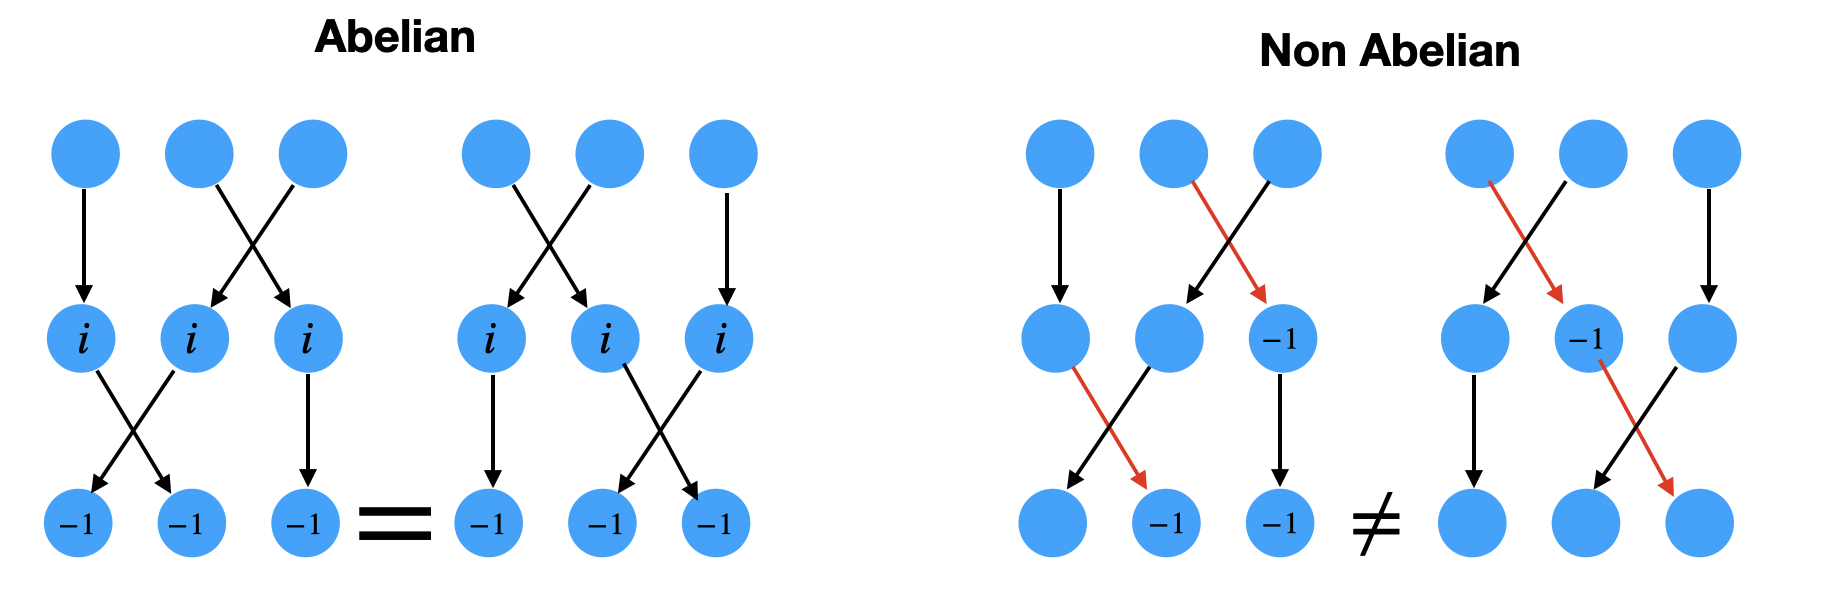
\includegraphics[width=0.8\linewidth]{imgs/AbVsNAb-Exchange.png}
  \caption{Exapmle of abelian and non abelian Exchange, With red arrows for the non-abelian $-1$ exchange path}
  \label{fig:AbVsNAb-Exchange}
\end{figure}
This allows us to perform braiding on non abelian Anyons. 
\subsubsection{Braid Group $\mathcal{B}_n$}\label{sec:braidGroup}
The exchange of such non-abelian particles can depend on the order of exchange. The Braid Group from Mathematics describes this behaviour and predicts when the order of exchange does not change the outcome.
Intuitively, one can imagine the braid group $\mathcal{B}_n$ as  $n$ strands being braided. Mathematically, the braid group $\mathcal{B}_n$ is generated by $n-1$ generators $\sigma_i$ with $i \in \{1,2,...,n-1\}$.\\
\begin{figure}[H]
    \centering
    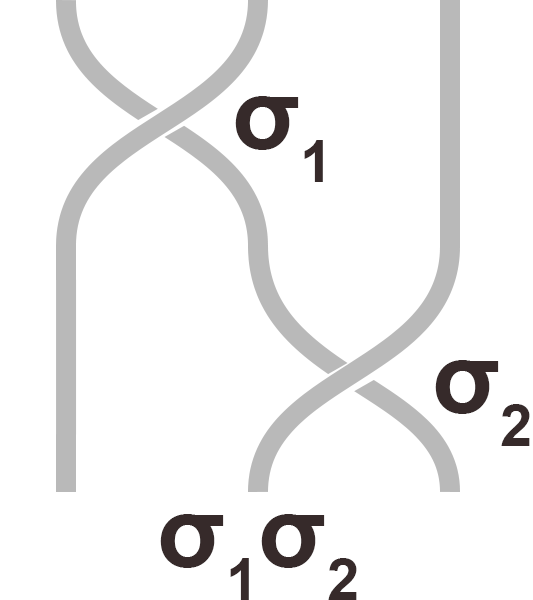
\includegraphics[height= 0.2\linewidth]{imgs/BraidGroup.png}
    \caption{Braiding of strands as symbolic interpretation of $\mathcal{B}_3$}
    \label{fig:Braid Group}
\end{figure}
The generators commute under certain conditions:
$$\sigma_i \sigma_j = \sigma_j \sigma_i \iff |i-j| > 1$$
\begin{figure}[H]
    \centering
    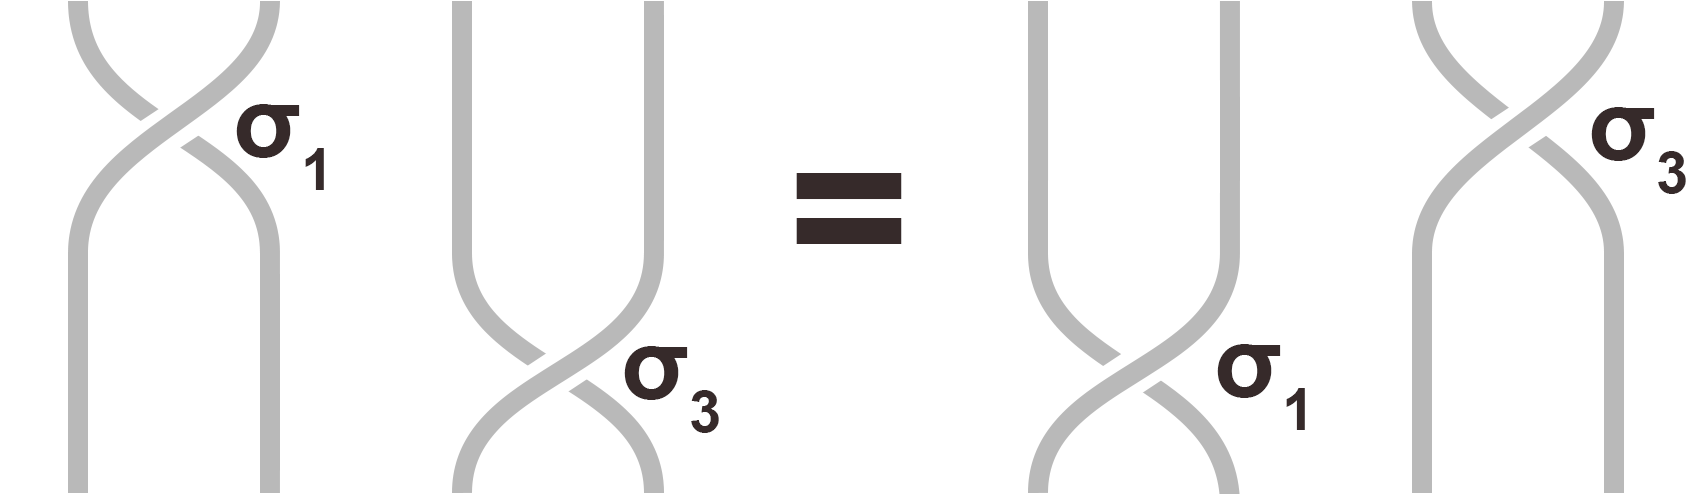
\includegraphics[height= 0.164\linewidth]{imgs/BraidGroup Identity 1.png}
    \caption{Braiding of distanced strands commutes}
    \label{fig:BnIdentity1}
\end{figure}
Visually, this corresponds to braiding two distanced strands \figref{fig:BnIdentity1}.
$$\sigma_i \sigma_{i+1} \sigma_i = \sigma_{i+1} \sigma_i \sigma_{i+1}$$ 
\begin{figure}[H]
    \centering
    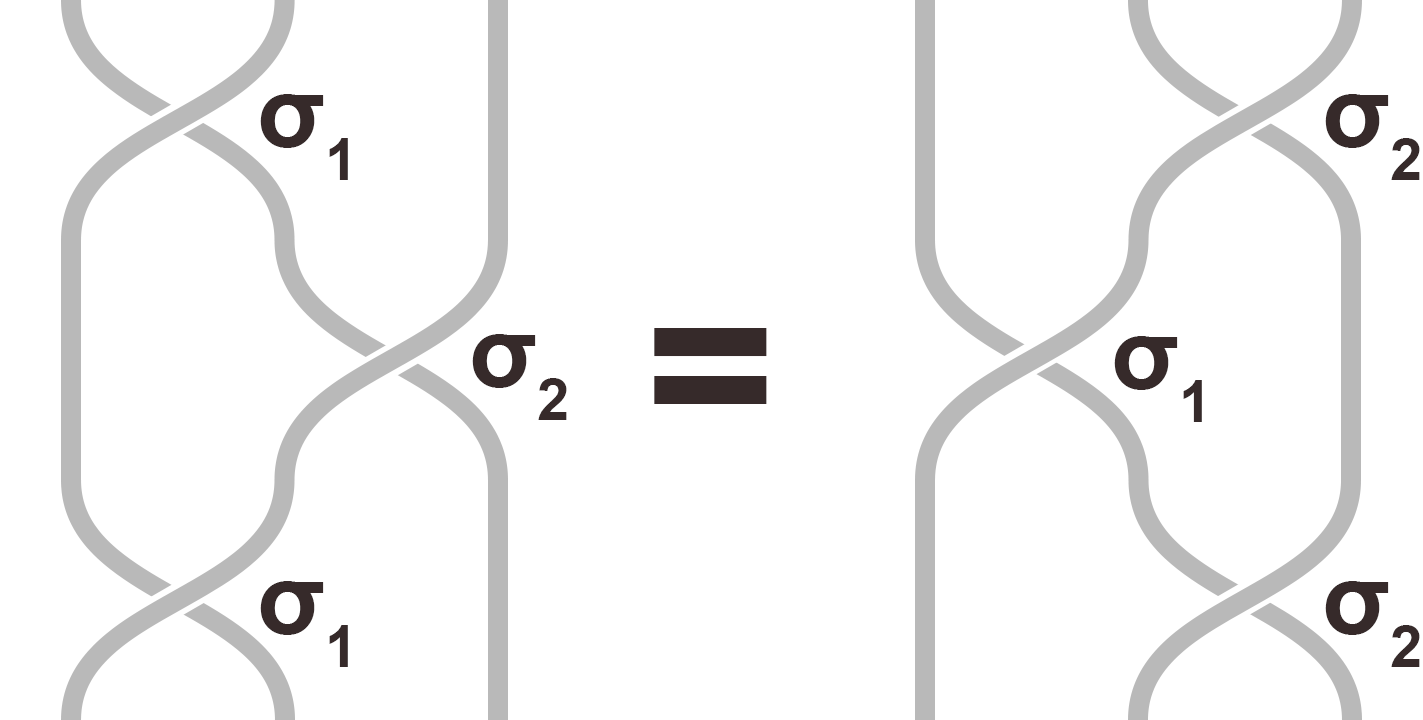
\includegraphics[height= 0.23\linewidth]{imgs/BraidGroup Identity 2.png}
    \caption{The middle strand can be moved smoothly from left to right to change $\sigma_1\sigma_2\sigma_1$ to $\sigma_2\sigma_1\sigma_2$ forming a homotopy.}
    \label{fig:BnIdentity2}
\end{figure}
The exchange statistics of $n$ non-abelian Anyons can be described by $\tau(\sigma) : \sigma \in \mathcal{B}_n$ elements in the Braid group $\mathcal{B}_n$.
\subsubsection{Topological Quantum Computing with Non-Abelian Anyons}
It can be demonstrated \cite{BRAVYI2002210} that the exchange statistics of non-abelian anyons are sufficient to perform Quantum Gate Computing. Elements in the braid group $\mathcal{B}_n$ correspond to quantum gates \cite{georgiev2017topological} e.g. \figref{fig:QGateBraids}:
\begin{figure}[H]
    \centering
    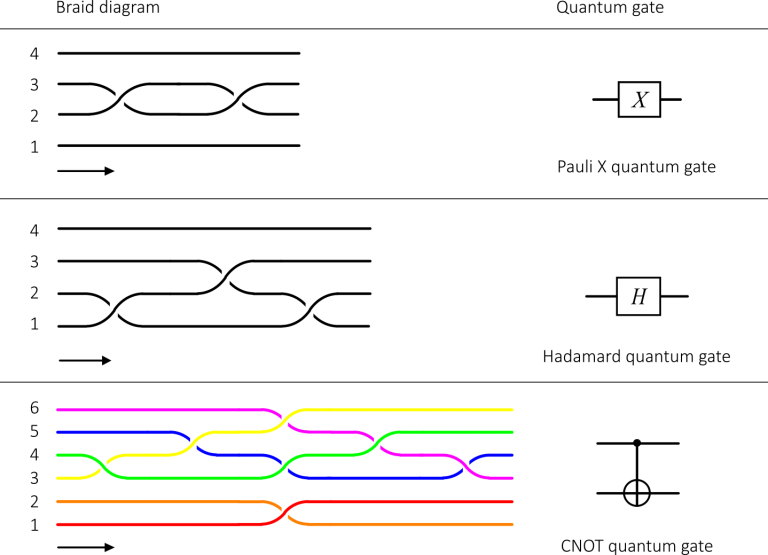
\includegraphics[width=0.8\textwidth]{imgs/QGateBraids.png}
    \caption{Examples of quantum gates and corresponding braid group elements from \cite{georgiev2017topological}}
    \label{fig:QGateBraids}
\end{figure}
However, we defined these exchange statistics for adiabatically slow exchange. For practical quantum computation, exchange statistics in finite time are necessary.
\end{document}